\section{Pianificazione}
	Alla luce delle scadenze riportate nella sezione 1.5 e alle scadenze interne si è deciso di dividere il progetto in cinque fasi:
	\begin{itemize}
		\item \textbf{Analisi};
		\item \textbf{Consolidamento dei requisiti};
		\item \textbf{Progettazione architetturale};
		\item \textbf{Progettazione di dettaglio e codifica};
		\item \textbf{Validazione e collaudo}.
	\end{itemize}
	Ognuna di queste cinque fasi sarà formata da diverse sottoattività mostrate nel corrispettivo diagramma di Gantt.

	\subsection{Analisi}
	\textbf{Periodo}: dal 26-11-2020 al 10-01-2021 \\
	La fase di Analisi è composta da sei attività che corrispondono alla produzione dei relativi documenti:
	\begin{itemize}
		\item \textbf{Studio di fattibilità}: Ogni capitolato proposto viene analizzato e discusso con i membri del gruppo. Ogni capitolato viene poi classificato in base alle preferenze e ai punti di iteresse riscontrati. Il capitolato che avrà riscosso più preferenze viene scelto come capitolato effetivo;
		\item \textbf{Norme di progetto}: Vengono definite le regole che il team dovrà rispettare durante lo sviluppo del progetto;
		\item \textbf{Piano di Progetto}: Si analizzato le attività, i compiti e le risorse che verranno distribuite tra i membri del team, presenta il calcolo del preventivo per la realizzazione del progetto;
		\item \textbf{Analisi dei requisiti}: Vengono studiati e analizzati i requisiti del capitolato scelto nello studio di fattibilità;
		\item \textbf{Piano di qualifica}: Durante questa attività si individuano le metodologie da usare per garantire la qualità del prodotto;
		\item \textbf{Glossario}: Questo documento viene redatto per definire la terminologia usata al fine di evitare ambiguità.
	\end{itemize}
	\subsubsection{Diagramma}
		\begin{figure}[H]
        		\centering
        		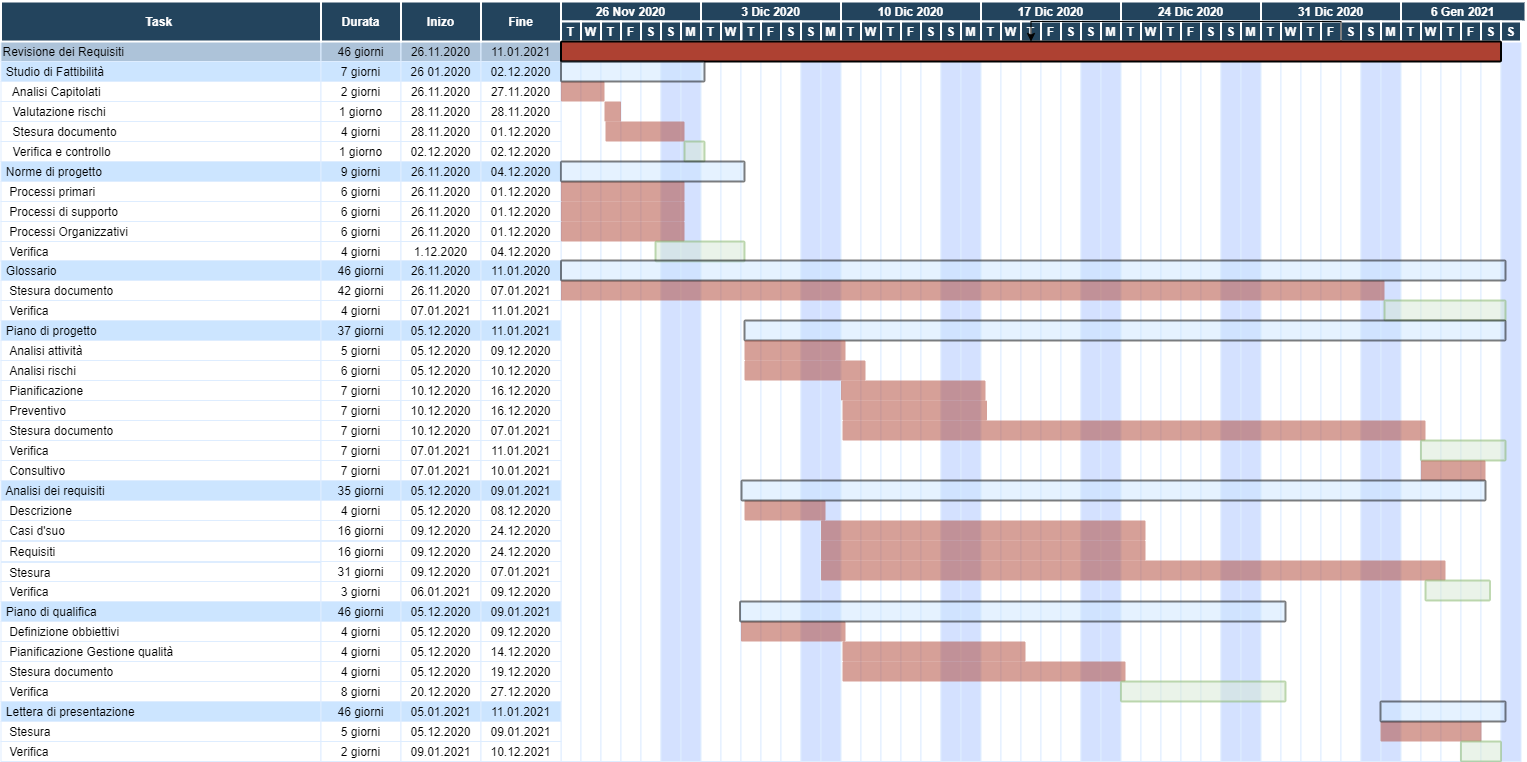
\includegraphics[width=0.8\textwidth]{source/img/analisiattivita.png}
        		\caption{Diagramma di Gantt dell'attività di analisi}
    		\end{figure}

	\subsection{Consolidamento dei requisiti}
	\textbf{Periodo}: dal 12-01-2021 al 18-01-2021 \\
	La fase di consolidamento dei requisiti è intermedia tra la fine della'attività di Analisi e il giorno della presentazione della Revisione dei Requisiti. \\
	Durante la seguente fase si svolgeranno attività di consolidamento dei requisiti osservati nella fase precedente e verrà preparata la presentazione per la Revisione dei Requisiti.
	
	\subsubsection{Diagramma}
		\begin{figure}[H]
        		\centering
        		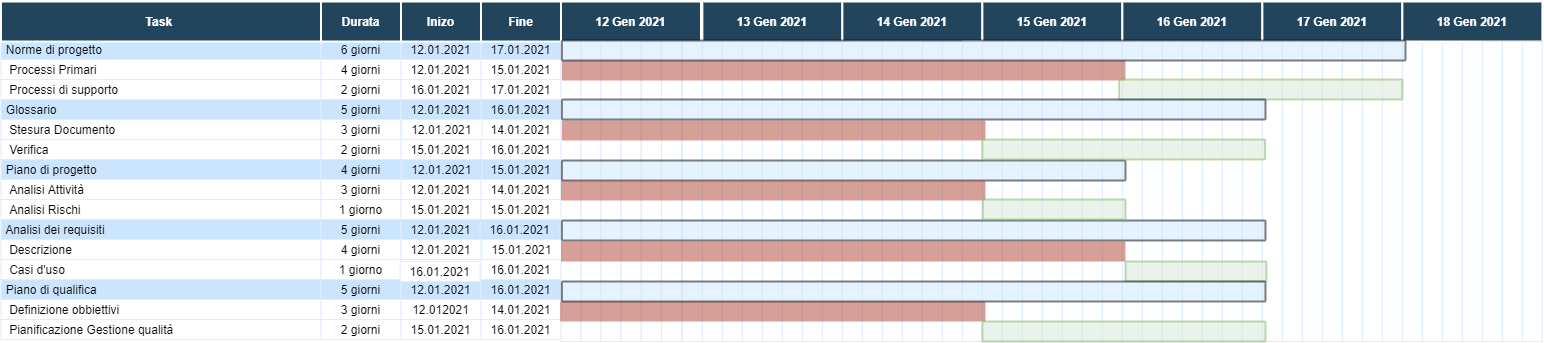
\includegraphics[width=0.8\textwidth]{source/img/Consolidamento_Requisiti.png}
        		\caption{Diagramma di Gantt dell'attività di consolidamento requisiti}
    		\end{figure}
	
	\subsection{Progettazione architetturale}
	\textbf{Periodo}: dal 19-01-2021 al 01-03-2021 \\
	Successivamente alla presentazione della Revisione dei Requisiti inizia la fase di progettazione architetturale che terminerà con la consegna della Revisione di Progettazione, lo scopo di questo periodo è l'individuazione di una soluzione architetturale che soddisfi i seguenti requisiti:
	\begin{itemize}
		\item \textbf{Technology Baseline}: Verrà stilato l'allegato tecnico nel quale verranno individuati i design pattern che verranno adottati nello sviluppo del progetto. Inoltre verrà redatto il Proof Of Concept da consegnare al committente;
		\item \textbf{Incremento di controllo}: Se necessarrio vengono migliorati i documenti consegnati durante la fase iniziale;
		\item \textbf{Incremento di sviluppo}: I documenti prodotti saranno aggiornati per rispecchiare l'attuale andamento del progetto.
	\end{itemize}
	
	\subsubsection{Diagramma}
		\begin{figure}[H]
        		\centering
        		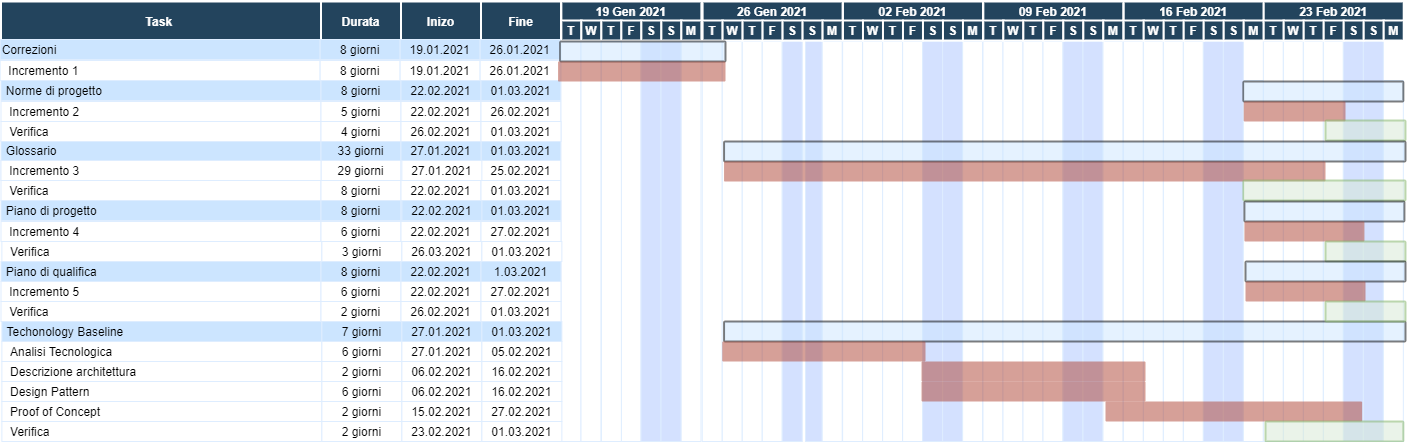
\includegraphics[width=0.8\textwidth]{source/img/Progettazione_architetturale.png}
        		\caption{Diagramma di Gantt dell'attività di progettazione architetturale}
    		\end{figure}
	\subsubsection{Tabella Incrementi}
		\begin{center}
    			\begin{tabular}{ | l | p{5cm} | p{8cm} |}
   			 \hline
    			Nome & Periodo & Descrizione \\ \hline
    			Incremento 1 & 19-01-2021 al 26-01-2021 & Ricevuto il feedback del committente i prodotti verranno aggiornati per risolvere le problematiche riscontrate. \\ \hline
    			Incremento 2 & 22-02-2021 al 01-03-2021 & Il documento Norme di Progetto verrà aggiornato per rispecchiare l'attuale situazione del progetto \\ \hline
    			Incremento 3 & 22-02-2021 al 01-03-2021 & Il documento Glossario verrà aggiornato per rispecchiare l'attuale situazione del progetto \\ \hline
			Incremento 4 & 22-02-2021 al 01-03-2021 & Il documento Piano di progetto verrà aggiornato per rispecchiare l'attuale situazione del progetto \\ \hline
			Incremento 5 & 22-02-2021 al 01-03-2021 & Il documento Piano di qualifica verrà aggiornato per rispecchiare l'attuale situazione del progetto \\ \hline
    			\end{tabular}
		\end{center}
	
	\subsection{Progettazione di dettaglio e codifica}
	\textbf{Periodo}: dal 02-03-2021 al 02-04-2021 \\
	Col termine della Revisione di Progettazione, inizia la fase di progettazione di dettaglio e codifica e terminerà con la Revisione di Qualifica, la seguente fase è composta da nuovi incrementi e attività:
	\begin{itemize}
		\item \textbf{Incremento e verifica}: Se necessario verranno migliorati i documenti consegnati durante la fase precedente;
		\item \textbf{Product Baseline}: Vengono studiati i design pattern, classi e attività necessarie alla codifica;
		\item \textbf{Specifica Tecnica}: Realizzazione di un documento contenente le specifiche del prodotto motivandone la scelta;
		\item \textbf{Codifica};
		\item \textbf{Manuale Utente}: Redazione del manuale utente del prodotto.
	\end{itemize}
	
	\subsubsection{Diagramma}
		\begin{figure}[H]
        		\centering
        		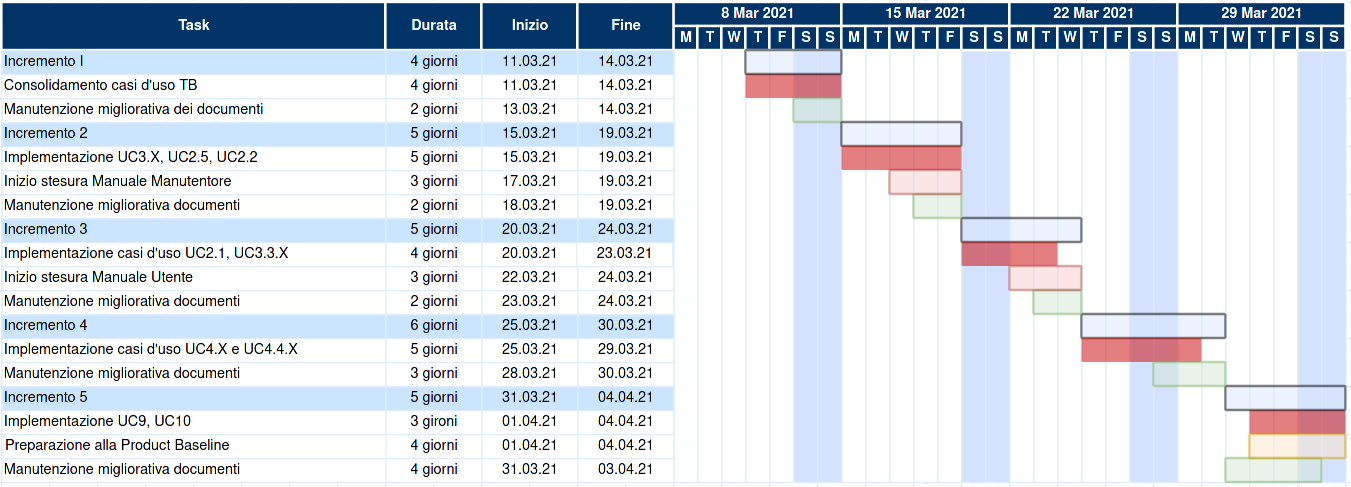
\includegraphics[width=0.8\textwidth]{source/img/Progettazionedettaglio_codifica.png}
        		\caption{Diagramma di Gantt dell'attività di progettazione di dettaglio e codifica}
    		\end{figure}
	\subsubsection{Tabella Incrementi}
		\begin{center}
    			\begin{tabular}{ | l | p{5cm} | p{8cm} |}
   			 \hline
    			Nome & Periodo & Descrizione \\ \hline
    			Incremento 1 & 02-03-2021 al 07-03-2021 & Ricevuto il feedback del committente i prodotti verranno aggiornati per risolvere le problematiche riscontrate. \\ \hline
    			Incremento 2 & 26-03-2021 al 01-04-2021 & Il documento Norme di Progetto verrà aggiornato per rispecchiare l'attuale situazione del progetto \\ \hline
    			Incremento 3 & 08-03-2021 al 01-04-2021 & Il documento Glossario verrà aggiornato per rispecchiare l'attuale situazione del progetto \\ \hline
			Incremento 4 & 23-03-2021 al 01-04-2021 & Il documento Piano di progetto verrà aggiornato per rispecchiare l'attuale situazione del progetto \\ \hline
			Incremento 5 & 26-03-2021 al 01-04-2021 & Il documento Piano di qualifica verrà aggiornato per rispecchiare l'attuale situazione del progetto \\ \hline
			Incremento 6 & 26-03-2021 al 01-04-2021 & Il documento Technology Baseline verrà aggiornato per rispecchiare l'attuale situazione del progetto \\ \hline
    			\end{tabular}
		\end{center}

	\subsection{Validazione e Collaudo}
	\textbf{Periodo}: dal 03-03-2021 al 03-04-2021 \\
	Ultima fase del progetto che terminerà con la Revisione di Accettazione, la seguente fase è composta da incrementi e nuove attività da svolgere:
	\begin{itemize}
		\item \textbf{Incremento e verifica}: Se necessario verranno migliorati i documenti consegnati durante la fase precedente;
		\item \textbf{Validazione e Collaudo}: Si eseguono i test finali di collaudo dell'applicazione nella sua interezza.
	\end{itemize}
	
	\subsubsection{Diagramma}
		\begin{figure}[H]
        		\centering
        		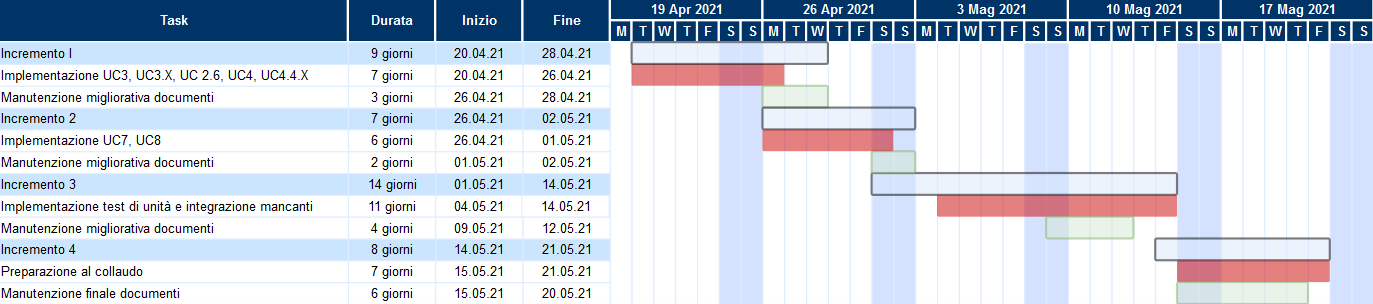
\includegraphics[width=0.8\textwidth]{source/img/Validazione_collaudo.png}
        		\caption{Diagramma di Gantt dell'attività di validazione e collaudo}
    		\end{figure}
	\subsubsection{Tabella Incrementi}
		\begin{center}
    			\begin{tabular}{ | l | p{5cm} | p{8cm} |}
   			 \hline
    			Nome & Periodo & Descrizione \\ \hline
    			Incremento 1 & 03-04-2021 al 08-04-2021 & Ricevuto il feedback del committente i prodotti verranno aggiornati per risolvere le problematiche riscontrate. \\ \hline
    			Incremento 2 & 24-03-2021 al 02-04-2021 & Il documento Glossario verrà aggiornato per rispecchiare l'attuale situazione del progetto \\ \hline
			Incremento 3 & 24-03-2021 al 02-04-2021 & Il documento Piano di progetto verrà aggiornato per rispecchiare l'attuale situazione del progetto \\ \hline
    			\end{tabular}
		\end{center}
